\documentclass[11pt,a4paper]{article}

\usepackage[T1]{fontenc}
\usepackage[utf8]{inputenc}
\usepackage{lmodern}
\usepackage{amsmath}
\usepackage[margin=2.25cm]{geometry}
\usepackage{graphicx}
\usepackage{booktabs}
\usepackage{array}
\usepackage{xcolor}
\usepackage{float}
\usepackage{caption}
\usepackage{fancyhdr}
\usepackage[hidelinks]{hyperref}

\definecolor{sourceRed}{RGB}{190,45,45}
\definecolor{traceGold}{RGB}{190,125,0}
\definecolor{targetBlue}{RGB}{35,85,190}
\definecolor{heading}{RGB}{36,54,82}

\pagestyle{fancy}
\fancyhf{}
\lhead{Advanced Software Engineering}
\rhead{Homework 5}
\cfoot{\thepage}
\setlength{\headheight}{14pt}

\captionsetup{font=small,labelfont=bf}
\setlength{\parindent}{0pt}
\setlength{\parskip}{0.65em}
\setlength{\emergencystretch}{2em}

\title{
    \vspace{-1.2cm}
    \textcolor{heading}{\Huge\bfseries Homework 5}\\[0.35cm]
}
\author{Matteo Carrese}
\date{}

\begin{document}

\maketitle


\section{Assignment and objective}

The assignment is to construct a Triple Graph Grammar (TGG) for transforming
Use Case Diagrams into Class Diagrams with AGG. The proposed solution focuses
on the main structural information of a use case model and keeps the grammar
small enough to be inspected and executed step by step.

A TGG works with three connected graphs:

\begin{itemize}
    \item the \textbf{source graph} contains the Use Case Diagram;
    \item the \textbf{correspondence graph} records the mappings;
    \item the \textbf{target graph} contains the generated Class Diagram.
\end{itemize}

The triple structure can be written as

\[
S \xleftarrow{\;s\;} C \xrightarrow{\;t\;} T,
\]

where $S$ is the source model, $C$ is the correspondence model, and $T$ is the
target model.

\section{Transformation mapping}

\begin{table}[H]
\centering
\begin{tabular}{>{\raggedright\arraybackslash}p{0.27\textwidth}
                >{\raggedright\arraybackslash}p{0.31\textwidth}
                >{\raggedright\arraybackslash}p{0.27\textwidth}}
\toprule
\textbf{Source} & \textbf{Correspondence} & \textbf{Target} \\
\midrule
\textcolor{sourceRed}{Actor} & \textcolor{traceGold}{Actor2Class} &
\textcolor{targetBlue}{Class} \\
\textcolor{sourceRed}{UseCase} & \textcolor{traceGold}{UseCase2Operation} &
\textcolor{targetBlue}{Operation} \\
\textcolor{sourceRed}{participates} &
\textcolor{traceGold}{Association2Ownership} &
\textcolor{targetBlue}{owns} \\
\bottomrule
\end{tabular}
\caption{The three mappings implemented by the grammar.}
\end{table}

The value of the source \texttt{name} attribute is copied to the generated
target element. As a result, an actor named \texttt{Customer} generates a
class named \texttt{Customer}, while a use case named \texttt{Place order}
generates an operation with the same name.

\clearpage
\section{Triple type graph}

The AGG type graph defines which nodes and edges may appear in the three
domains. Source types are red, correspondence types are yellow, and target
types are blue. This visual convention makes every part of the transformation
easy to identify.

\begin{figure}[H]
    \centering
    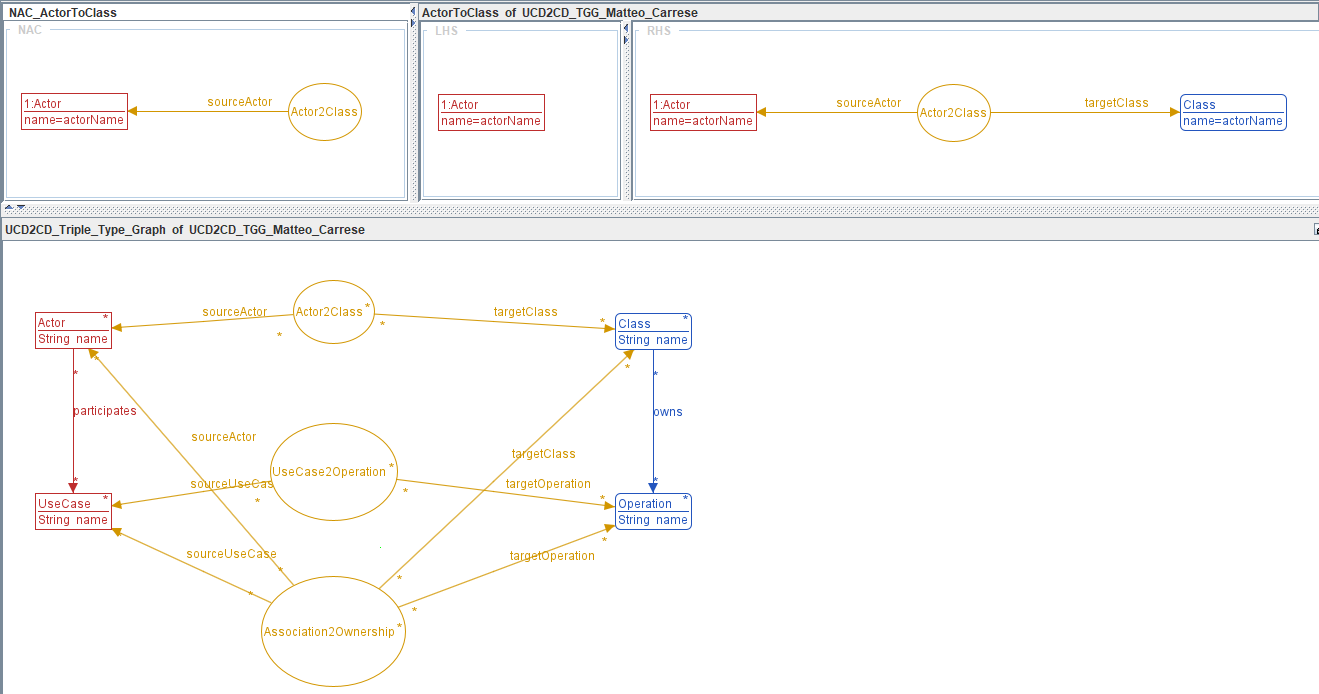
\includegraphics[width=\textwidth,trim=0 0 450 157,clip]{images/01_type_graph.png}
    \caption{The complete triple type graph in AGG.}
\end{figure}

The source graph contains \texttt{Actor}, \texttt{UseCase}, and the directed
edge \texttt{participates}. The target graph contains \texttt{Class},
\texttt{Operation}, and the edge \texttt{owns}. Three correspondence types
connect the two sides.

The correspondence graph is not only a visual aid. It allows a rule to locate
the exact target object generated from a source object. For example, the third
rule follows an \texttt{Actor2Class} node instead of searching for a class only
by its name.

\section{Transformation rules}

The grammar contains three rules executed in layer order.

\subsection{ActorToClass}

The first rule matches an actor and creates a class with the same name. It also
creates an \texttt{Actor2Class} node connected to both objects. A Negative
Application Condition (NAC) prevents the rule from running if that actor has
already been transformed.

\subsection{UseCaseToOperation}

The second rule transforms each use case into an operation and creates a
\texttt{UseCase2Operation} trace. Its NAC prevents duplicate operations.


\subsection{AssociationToOwnership}

The third rule is applied after the actor and use case mappings exist. Its
left-hand side matches an actor, a use case, their \texttt{participates} edge,
and the corresponding class and operation.

\begin{figure}[H]
    \centering
    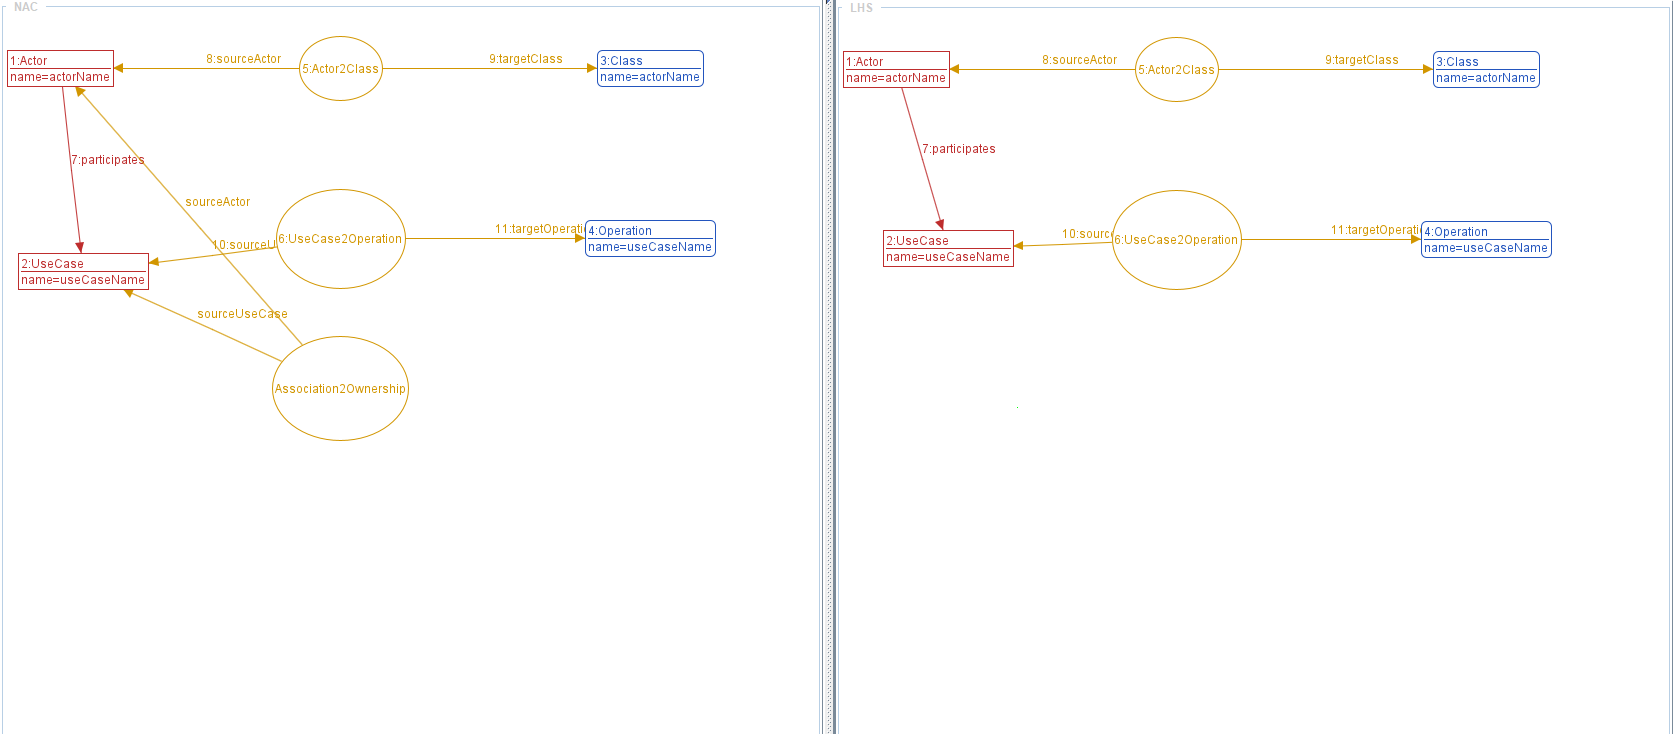
\includegraphics[width=\textwidth]{images/03_association_nac_lhs.png}
    \caption{The NAC and left-hand side of AssociationToOwnership.}
\end{figure}

The right-hand side preserves all matched objects and adds an
\texttt{Association2Ownership} trace together with the blue \texttt{owns}
edge from the class to the operation.

\begin{figure}[H]
    \centering
    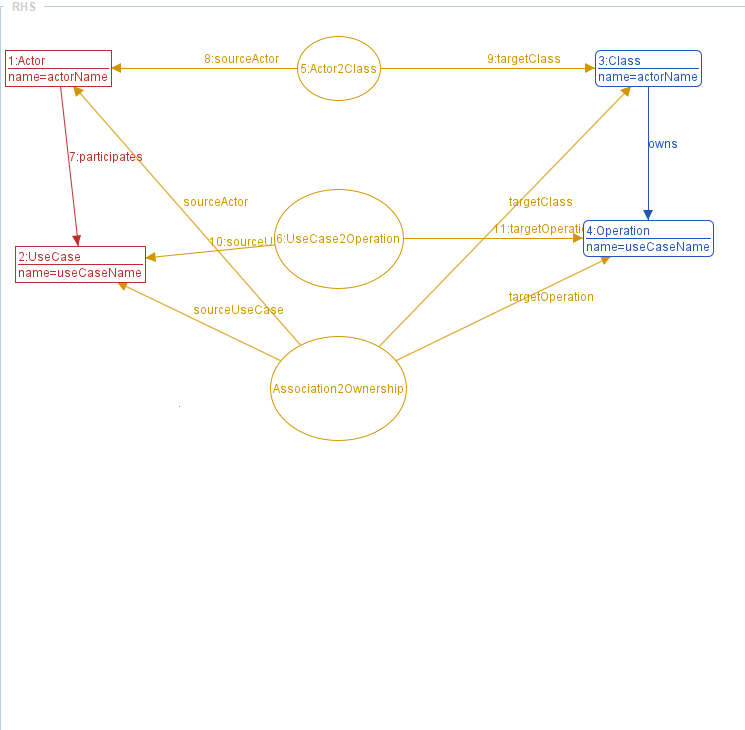
\includegraphics[height=0.40\textheight,trim=0 50 0 0,clip]{images/04_association_rhs.png}
    \caption{The right-hand side creates the trace and ownership relation.}
\end{figure}

The NAC checks that the association trace does not already exist. Therefore,
the same source association cannot generate the target ownership relation more
than once.

\clearpage
\section{Example transformation}

The initial host graph models a small online shop. The customer participates
in \texttt{Browse catalog} and \texttt{Place order}. The administrator
participates in \texttt{Manage catalog}.

\begin{figure}[H]
    \centering
    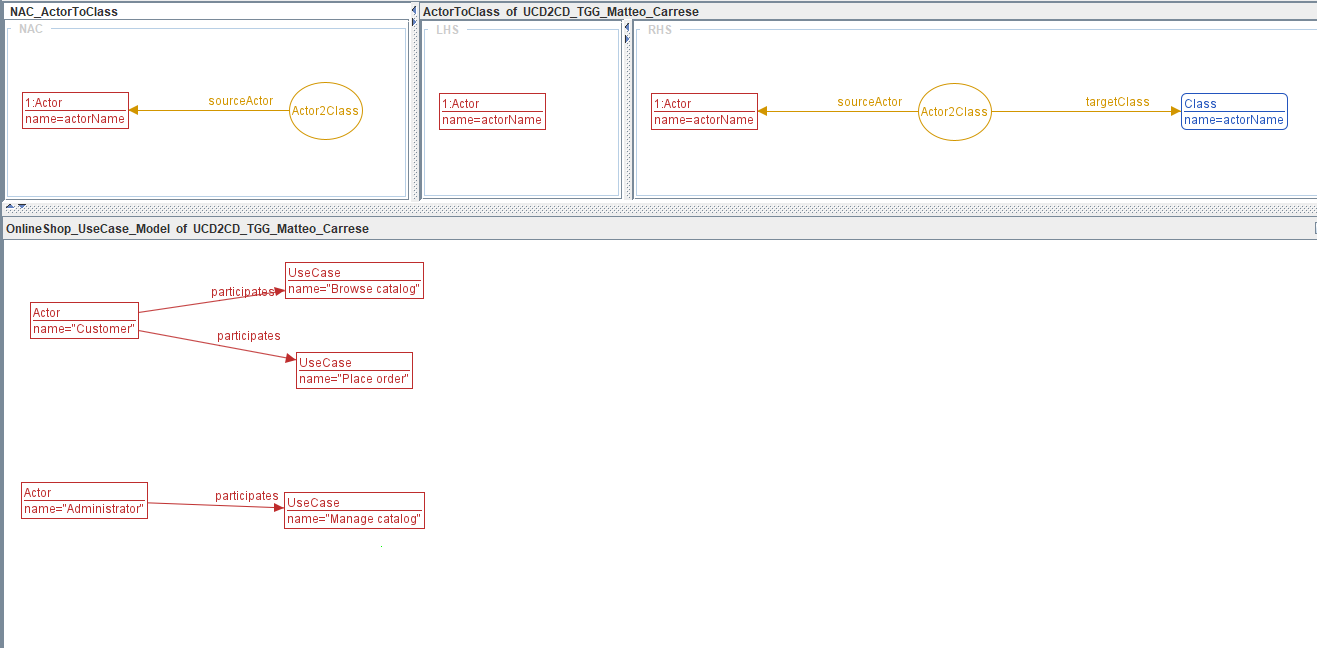
\includegraphics[width=0.78\textwidth,trim=0 70 605 155,clip]{images/02_initial_host_graph.png}
    \caption{The source-only host graph before transformation.}
\end{figure}

AGG applies the rules by layer:

\begin{enumerate}
    \item \texttt{ActorToClass} creates the two classes;
    \item \texttt{UseCaseToOperation} creates the three operations;
    \item \texttt{AssociationToOwnership} creates the three ownership edges.
\end{enumerate}

The source model is preserved. The new correspondence and target elements are
added to the same typed graph, allowing the complete transformation trace to
be inspected.

\clearpage
\begin{figure}[H]
    \centering
    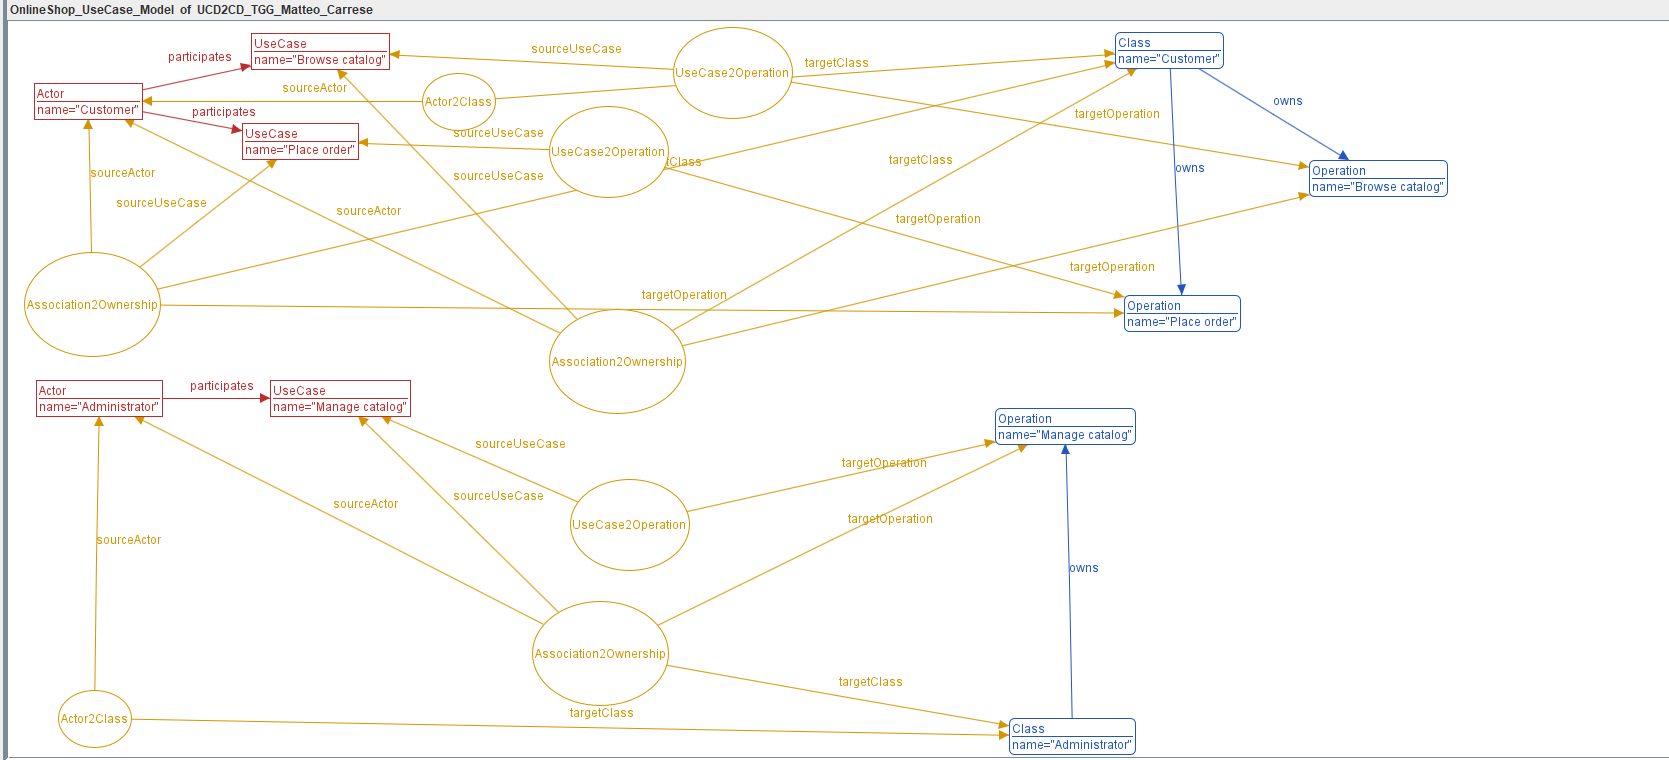
\includegraphics[width=\textwidth,trim=0 0 110 0,clip]{images/05_transformation_result.png}
    \caption{The host graph after the complete transformation.}
\end{figure}

The final target model contains the following information:

\begin{table}[H]
\centering
\begin{tabular}{ll}
\toprule
\textbf{Generated class} & \textbf{Owned operations} \\
\midrule
Customer & Browse catalog; Place order \\
Administrator & Manage catalog \\
\bottomrule
\end{tabular}
\caption{Resulting class diagram elements.}
\end{table}

The complete graph contains 18 nodes and 28 edges. These values include the
five source nodes, three source associations, the generated target objects,
all correspondence nodes, and their trace edges.

\section{Termination and correctness}

Each rule has one NAC. The NAC checks for the correspondence object created by
that rule. Once the trace exists, the rule cannot be applied again to the same
source pattern. This prevents duplicates and makes execution terminate after
all source elements have been processed.

The grammar was loaded and executed with AGG. All three layers completed, and
the resulting graph remained consistent with the type graph. Reapplying the
transformation does not create another class, operation, or ownership relation
for an already transformed element.

\section{Conclusion}

The grammar provides a simple but complete example of a model-to-model
transformation. It separates source, correspondence, and target concepts,
copies element names, preserves the original model, and prevents duplicate
results through NACs. Additional UML relations such as include, extend, and
generalization could be supported by adding new types and transformation rules
without changing the basic three-domain architecture.

\end{document}

